\documentclass{vldb}
\usepackage{graphicx}
\usepackage{balance}
\usepackage{multirow}
\usepackage{booktabs}



\begin{document}

\title{Strength in numbers? Modelling the impact of businesses on each other}

\numberofauthors{3} 

\author{
\alignauthor
Amir Abbas Sadeghian\\
       \email{amirabs@stanford.edu}
\alignauthor
Hakan Inan\\
       \email{inanh@stanford.edu}
\alignauthor 
Andres N\"otzli\\
       \email{noetzli@stanford.edu}
}

\maketitle

\begin{abstract}
Here goes nothing.
\end{abstract}

\section{Introduction}
In many cities, there is a small number of streets with a lot of restaurants.
Being in a street like this is a double-edged sword for the individual restaurant. 
On one side, it is valuable because it gets them the attention of potential customers for free. 
On the other hand, the restaurants are competing for customers with similar needs and the offerings are not free from overlap. \cite{pedregosa2011scikit}
Our hypothesis is that this balance is a function of the size of the cluster.
The bigger the cluster grows, the more customers start to search for a restaurant within this cluster, increasing the number of total customers of the cluster and emphasizing the symbiosis of the restaurants living in the cluster. 
At the same time, however, the number of potential customers is limited and as it nears saturation, the competitive nature of the relationship between the restaurants grows stronger.
The goal of our project is to test this hypothesis by finding clusters of restaurants in a dataset and to model how the individual restaurant is affected by being part of the cluster. 
Machine learning will play a crucial role in this process, from finding clusters of restaurants to model the impact on the individual restaurant. 
We will start by comparing clusters of different sizes but ideally we would like to find clusters where we can observe growth over time and the effect on the restaurants over this time period. If the project proves to be successful, it has the potential to offer a unique insight in the relationship between restaurants in such clusters.
To design and evaluate our model, we are planning to use the Yelp dataset. 

\section*{Main Objectives}
\begin{enumerate}
\item Business Clustering
\item Impact of a new business on a cluster
	\begin{itemize}
 	 \item Propose and test impact models
 	 \item Use machine learning techniques to predict the impact
  	\end{itemize}
	
\end{enumerate}

\section{The dataset}

Yelp is a website where users review businesses like restaurants. The dataset contains data for more than 40’000 businesses and more than 1 million of reviews. There is a rich set of attributes for each business and there is additional data like the number of checkins that can be used to model the popularity of a place.

Two data points that are missing from the dataset are the opening and the closing date of a business.
To compensate for the lack of information, we use a simple heuristic: We assume that the business opened on the date of the first comment and we assume that it has been closed on the date of the last comment if the last comment more than 2 months older than the newest comment in the dataset.
We argue that this is a reasonable choice because our project requires us to look at businesses with a reasonable number of ratings and in these cases the opening/closing date should be reasonably close to the date of the first and the last review.
Yelp is a website where users view and review businesses like restaurants. The dataset contains data from several cities and there is a rich set of attributes for each business. \\

\begin{minipage}[b]{0.45\linewidth}
\begin{itemize}
	\item[
\includegraphics{Yelp_logo.png}]42,153 businesses 
	\item[
\includegraphics{Yelp_logo.png}] 320,002 business attr.
    \item[
\includegraphics{Yelp_logo.png}] 31,617 check-in sets 
\end{itemize}
\end{minipage}
\begin{minipage}[b]{0.45\linewidth}
\begin{itemize}
    \item[
\includegraphics{Yelp_logo.png}] 252,898 users
    \item[
\includegraphics{Yelp_logo.png}] 403,210 tips 
    \item[
\includegraphics{Yelp_logo.png}] 1,125,458 reviews
\end{itemize}
\end{minipage}

\section{Preprocessing}
\subsection{Running average of ratings}
The running average of ratings plays an important role when predicting the correlation of two businesses.
The raw user ratings are highly noisy and relatively sparse.
Figure~\ref{fig:moving_average} depicts an example of a moving average for a business over time.
In addition, we filter out businesses with a low number of ratings.

\begin{figure}[h]
\centering
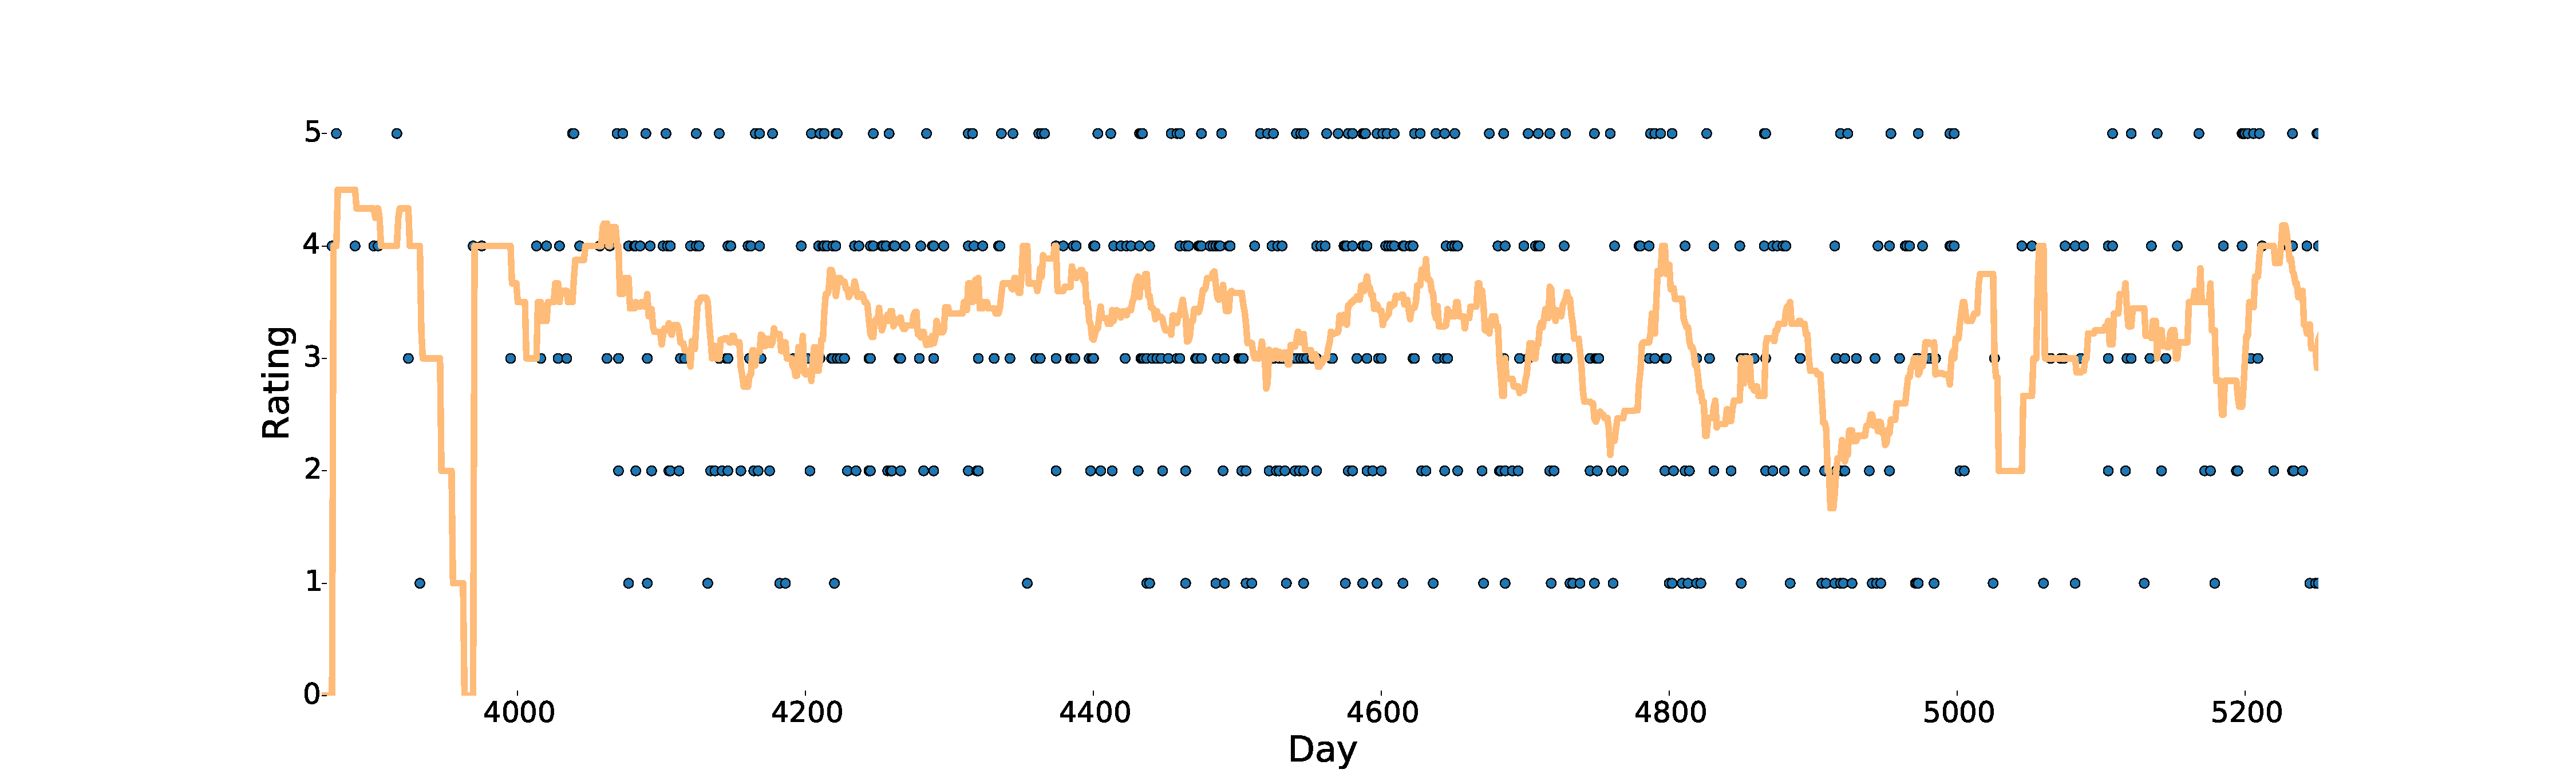
\includegraphics[width=\columnwidth]{moving_avg.pdf}
\caption{ Moving average of ratings for a specific business}
\label{fig:correlation}
\end{figure}

\subsection{Clustering}
We checked different clustering algorithms and for the same number of clusters, K-Means based on the geographic locations of businesses had the best result. The result of two clustering algorithms results are shown in Figure~\ref{fig:clusters}.

\begin{figure}[h]
\centering
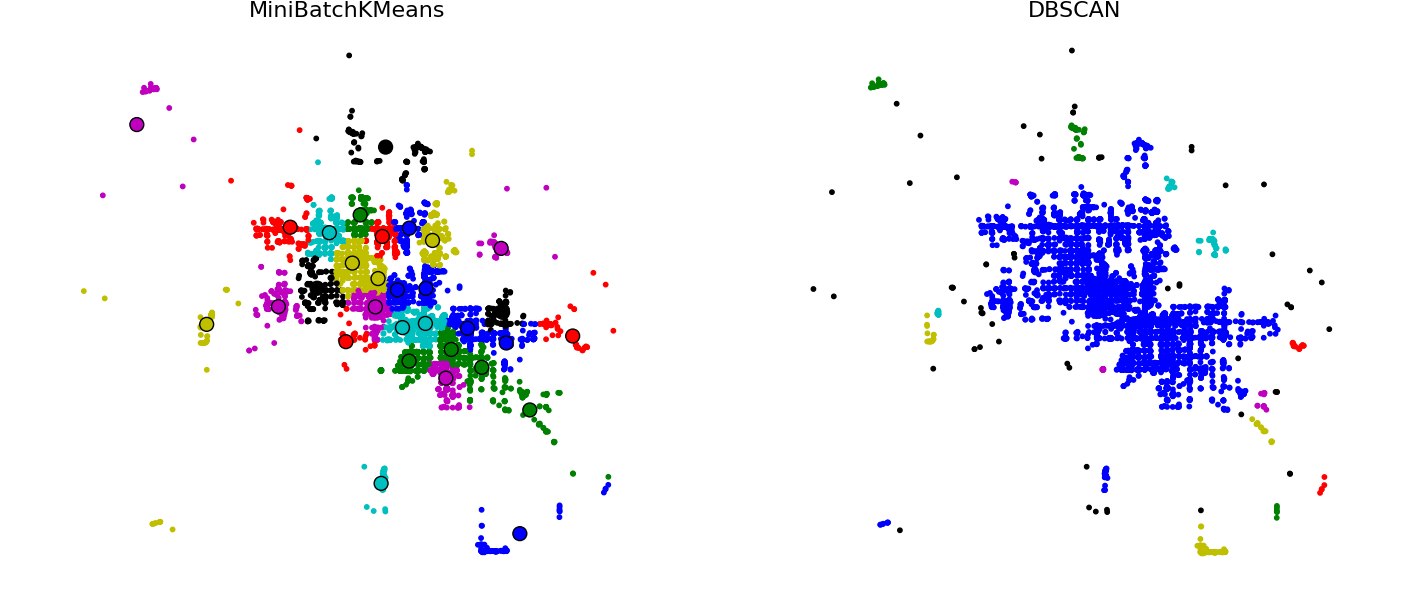
\includegraphics[width=\columnwidth]{clusters.png}
\caption{ K-Means and DBSCAN clustering}
\label{fig:correlation}
\end{figure}

As we previously described in the introduction, we are interested to look at clusters of businesses.
The first step in our project is thus to find a good way of clustering businesses.
We found that using zip codes to group businesses is ineffective as groups of businesses often span zip code boundaries.
We experimented with multiple clustering methods and ended up using k-means clustering with the geographical location as features because we are interested to observe interaction between businesses that are physically close to each other. Using k-means we are taking the advantage of clustering close businesses together and also putting far businesses that are not influencing each other into different clusters. In this case we can assume that the businesses in two different clusters are independent, and only businesses in one cluster influence each others behaviors. We will have a brief overview on the different clustering techniques used and a benchmark that reasons which one works the best in the case of our study.

\section{Feature selection}
In various domains, like text learning, image classification, and specially cases where there are many features compared to data samples feature selection techniques are used. The feature sets selected for our model plays an important role to define a better feature similarity measure which can lead to improvement of our prediction algorithms and also finding correlations between different businesses.
Once feature which is used to find the correlations of business ratings in section ~\ref{sec:correlation_of_ratings}, is the moving average of ratings stars. This feature give us an understanding of how a business was performing in a period of time and how the users rated that specific business in that time.


\section{Correlation of ratings}
\label{sec:correlation_of_ratings}
\begin{figure}
\centering
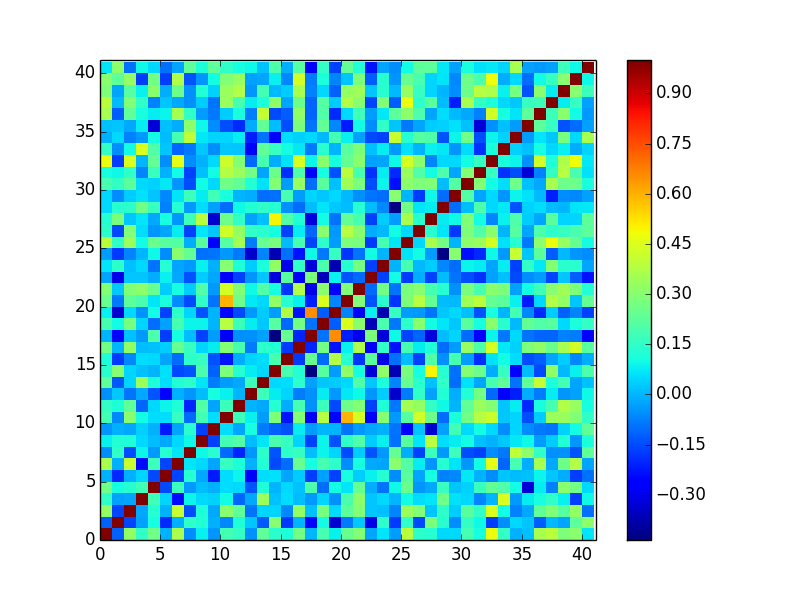
\includegraphics[width=\columnwidth]{cov_cluster_28}
\caption{Correlation between ratings of businesses in the same cluster}
\label{fig:correlation}
\end{figure}
After getting the clusters, we analyze the correlation of ratings between different businesses in the same cluster.
To do so, we first apply a Gaussian filter to the time series of ratings to smooth out local fluctuations in ratings. The correlation of the ratings is then given by:

\begin{align*}
    \rho_{XY} &= \frac{E(XY)}{\sqrt{E(X^2) E(Y^2)}} \\
    E(X) &= \frac{1}{n} \sum_{t = 0}^{n} r_t
\end{align*}

Where $r_t$ is the filtered rating.
In this step we discard all businesses with a low number of ratings because they provide not enough signal to get a good estimate for the correlation.

As Figure~\ref{fig:correlation} shows, there are a couple of cases with strong correlation.

\section{Features}
We found that a combination of geographical distance, price range difference, age, and business categories work best as features to describe the relationship between two businesses. The categories encode attributes of a restaurant like the type of food that it serves.

\section{Models}
All the analysis in the project was based on using the pairwise features outlined above for predicting pairwise metrics to be defined in what follows. Specifically, in this section we introduce 4 different metrics which we will henceforth call "pairwise impact metrics". 

\textit{NOTE:} Anything below is within a cluster



\subsection*{Conditional Mean Analysis}

\begin{figure}[h]
\centering
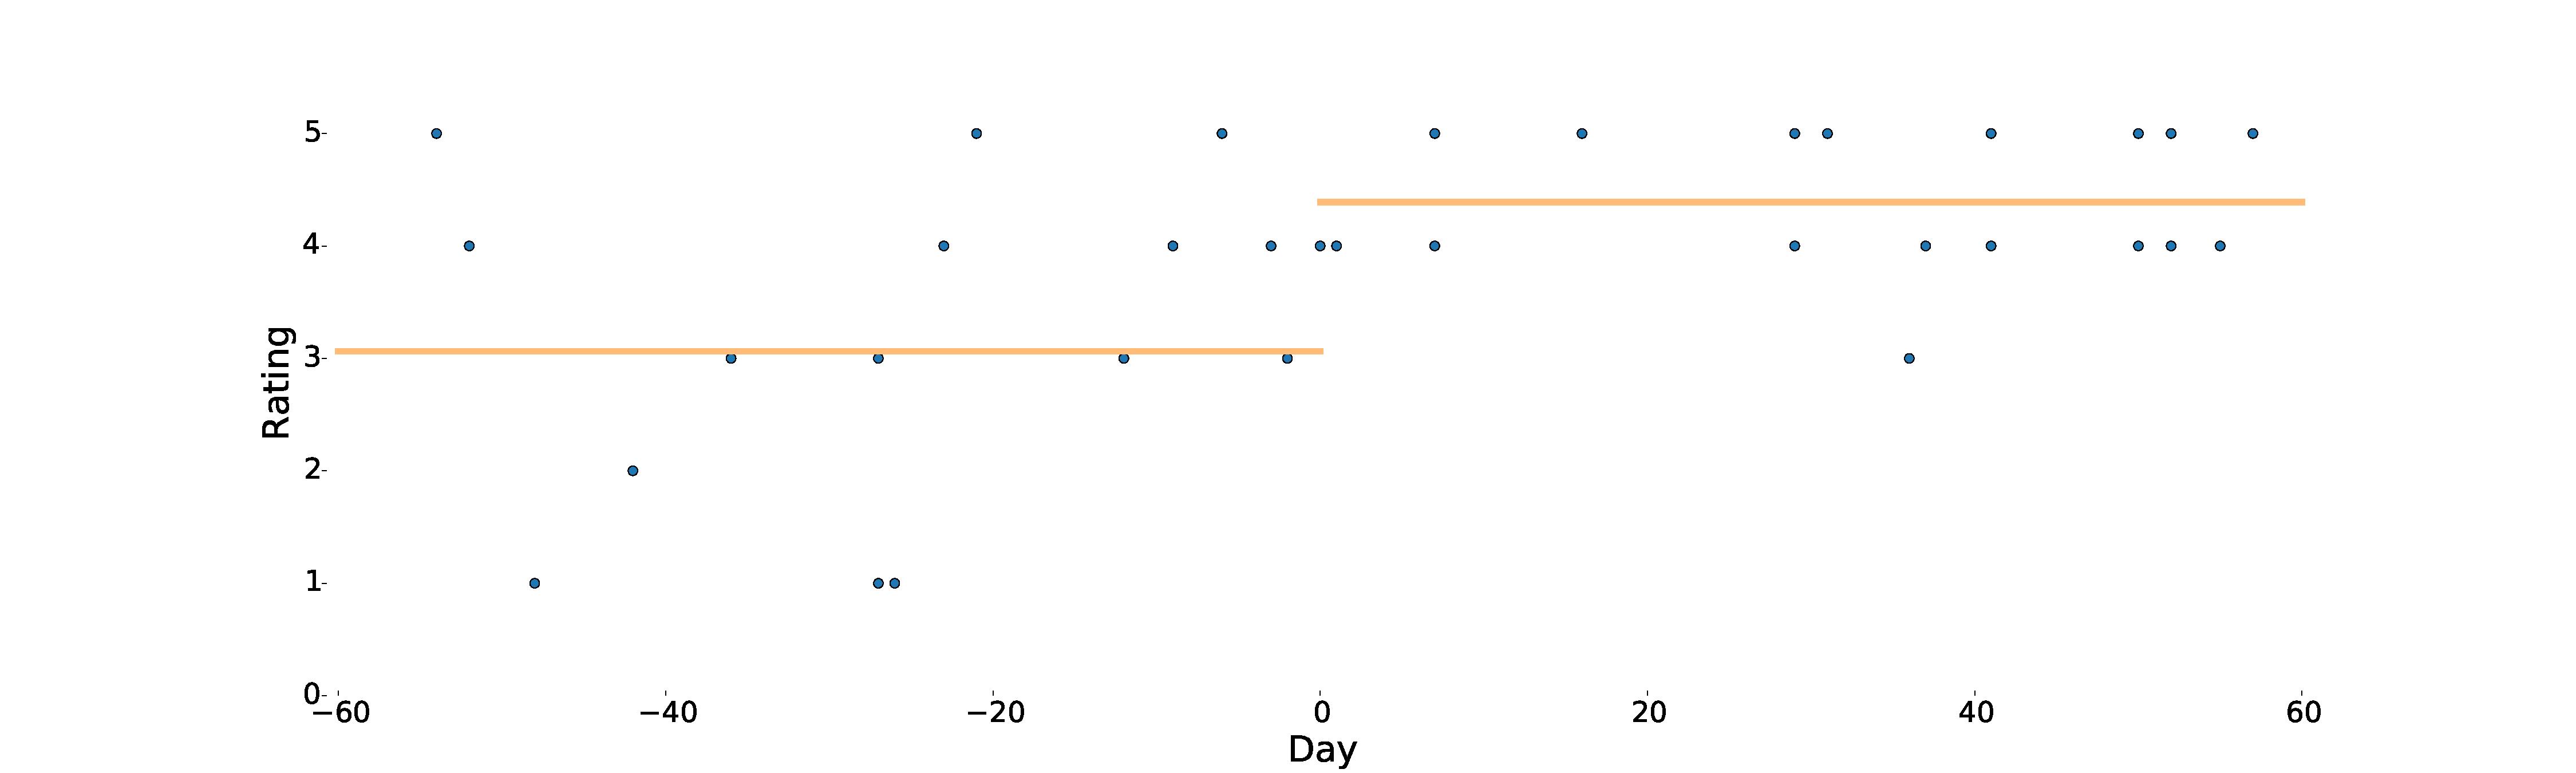
\includegraphics[width=\columnwidth]{mean.pdf}
\caption{Example mean analysis for a pair of businesses}
\end{figure}

\textbf{\textit{Hypothesis}} : Opening of a new business has an impact on the mean of ratings of the  businesses nearby.\\
\textbf{\textit{Proxy}} : Calculate the mean ratings of the nearby businesses before and after a new business opens, and get a comparative metric.\\
\textbf{\textit{Expected results}} : The change in the conditional means of the existing businesses may be predicted using the attributes of the existing businesses and the new business. \\ \\
\begin{small}
The mean ratings  were calculated as follows:\\ \\
$E_{before}(b)=\frac{1}{R_b} \sum_{x: -M+d_0\le d_x \le d_0} r_x(b),\\
E_{after}(b)=\frac{1}{R_a} \sum_{x: d_0\le d_x \le d_0+M} r_x(b)\\ \\
d_x = \small\text{day of the review x }, \\
d_0 = \small\text{opening day of the new business}, \\
r_x = \small\text{rating of review x}, \\
M = \small\text{number of days to average over}\\ $

For this analysis, we needed a date of opening for the businesses. However, we didn't have the true opening dates in the dataset, and we estimated them to be the dates of the first review for the businesses. \\
The pairwise impact metric in the conditional mean analysis was determined as $E_{before} - E_{after}$.

\label{eqn:condMean}
\end{small}



\subsection*{Trend Analysis}
\begin{figure}[h]
\centering
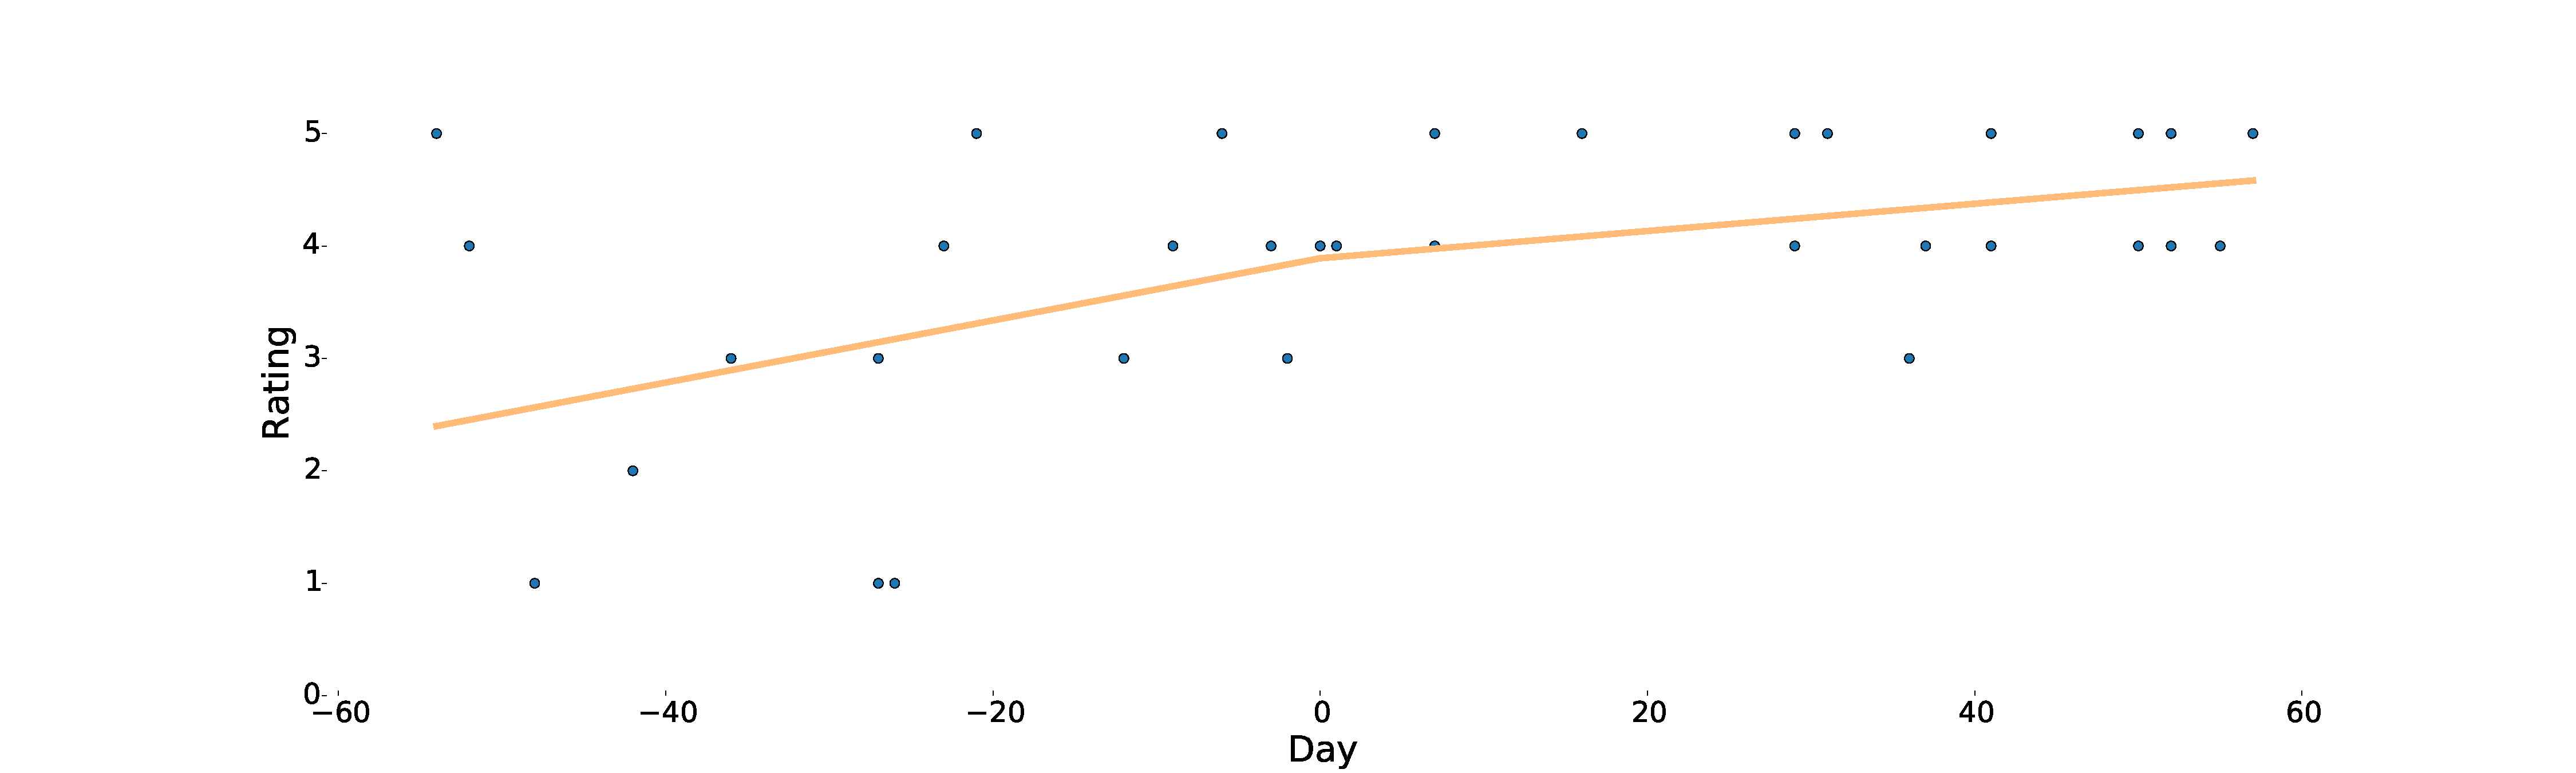
\includegraphics[width=\columnwidth]{trend.pdf}
\caption{Example trend analysis for a pair of businesses}
\end{figure}

\textbf{\textit{Hypothesis}} : Opening of a new business has an impact on the trends of ratings of the businesses nearby.\\
\textbf{\textit{Proxy}} : Fit separate lines for the ratings of a business both before and after a new business opens in the neighborhood. Calculate a metric based on the difference in the slopes of the two lines.\\
\textbf{\textit{Expected results}} : The change in the trends of the existing businesses with respect to the launching  of a new business in the neighborhood may be predicted using the attributes of the existing businesses and the new business. 

First, we estimated the opening date of the businesses as explained in the previous subsection. Then, for each pair of businesses we fit two lines for the ratings of the older business around the origin (the estimated opening date of the newer business) within a specified time window, imposing that the lines touch at the origin . Specifically, we are solving the following least squares problem:
\begin{equation*}
 \left [\begin{array}{ccc}x_{before} & 0 & 1 \\
 0 & x_{after} & 1 \end{array} \right ] 
  \left [\begin{array}{c}s_1 \\ s_2 \\ c \end{array} \right ] 
 =  \left [\begin{array}{c}y_{before} \\ y_{after} \end{array} \right ] ,
\end{equation*}
where $x_{before}$  ($x_{after}$) is a vector of the days of filtered ratings of the older business before (after) the newer business opens, $y_{before}$  ($y_{after}$) is a vector of filtered ratings of the older business before  (after) the newer business opens, $s_1$  ($s_2$) is the slope of the line fitted to the ratings of the older business before  (after) the newer business opens, and $c$ is the common intercept for the two lines. One thing to note here is that the elements of $x_{before}$ and $x_{after}$ are shifted such that the last element of $x_{before}$ is 0 and the first element of $x_{after}$ is 1.

The pairwise impact metric was determined to be the difference in the angles of the two slopes. 

\subsection*{General Trend Analysis}

\begin{figure}[h]
\centering
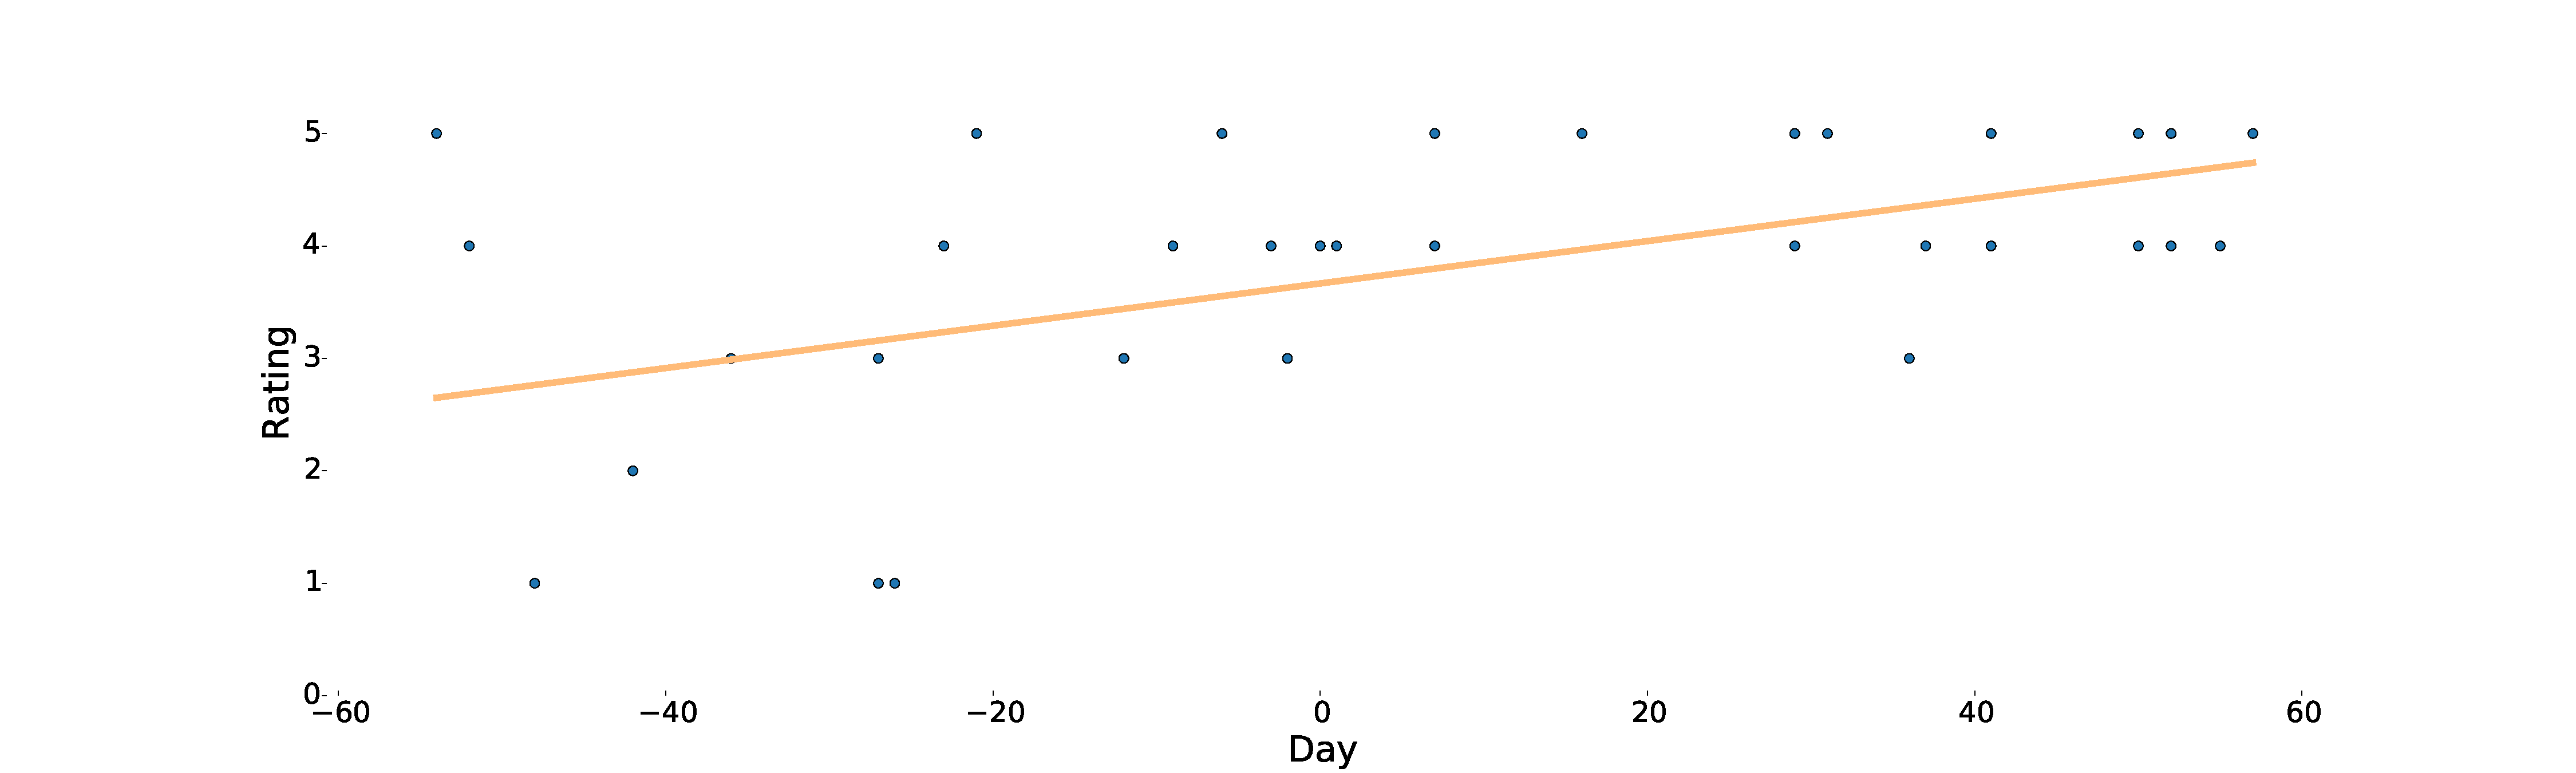
\includegraphics[width=\columnwidth]{gen_trend.pdf}
\caption{   Example general trend analysis for a pair of businesses}
\end{figure}

\textbf{\textit{Hypothesis}} : The exact opening date is not known and since prediction is noisy, the trend analysis might fail. The general trends of the existing businesses around a rough estimate of the opening time of a new business may reflect (with less noise compared to the trend analysis) the impact of the new business on them.\\
\textbf{\textit{Proxy}} : Fit a single line for the ratings of a business around the estimated opening date of a newly opened business in the neighborhood. Determine if the business has an increasing or a decreasing trend based on the slope of the line.\\
\textbf{\textit{Expected results}} : The general trends of the existing businesses around the launching date of a new business in the neighborhood may be predicted using the attributes of the existing businesses and the new business. 

The method to apply was very similar to that for the trend analysis, with the distinction being that for general trend analysis we fitted a single line for the whole time window and calculated a single slope. Mathematically, we calculated the least square solution to the following equation:
\begin{equation*}
 \left [\begin{array}{c}x_{before} \\ x_{after}  \end{array} \right ] 
  \left [\begin{array}{c}s \\ c \end{array} \right ] 
 =  \left [\begin{array}{c}y_{before} \\ y_{after} \end{array} \right ] ,
\end{equation*}
with everything except for $s$ is as defined in the previous subsection. $s$ is the slope to the fitted line for the whole time window .


\subsection*{Correlation Analysis}
\begin{figure}[h]
\centering
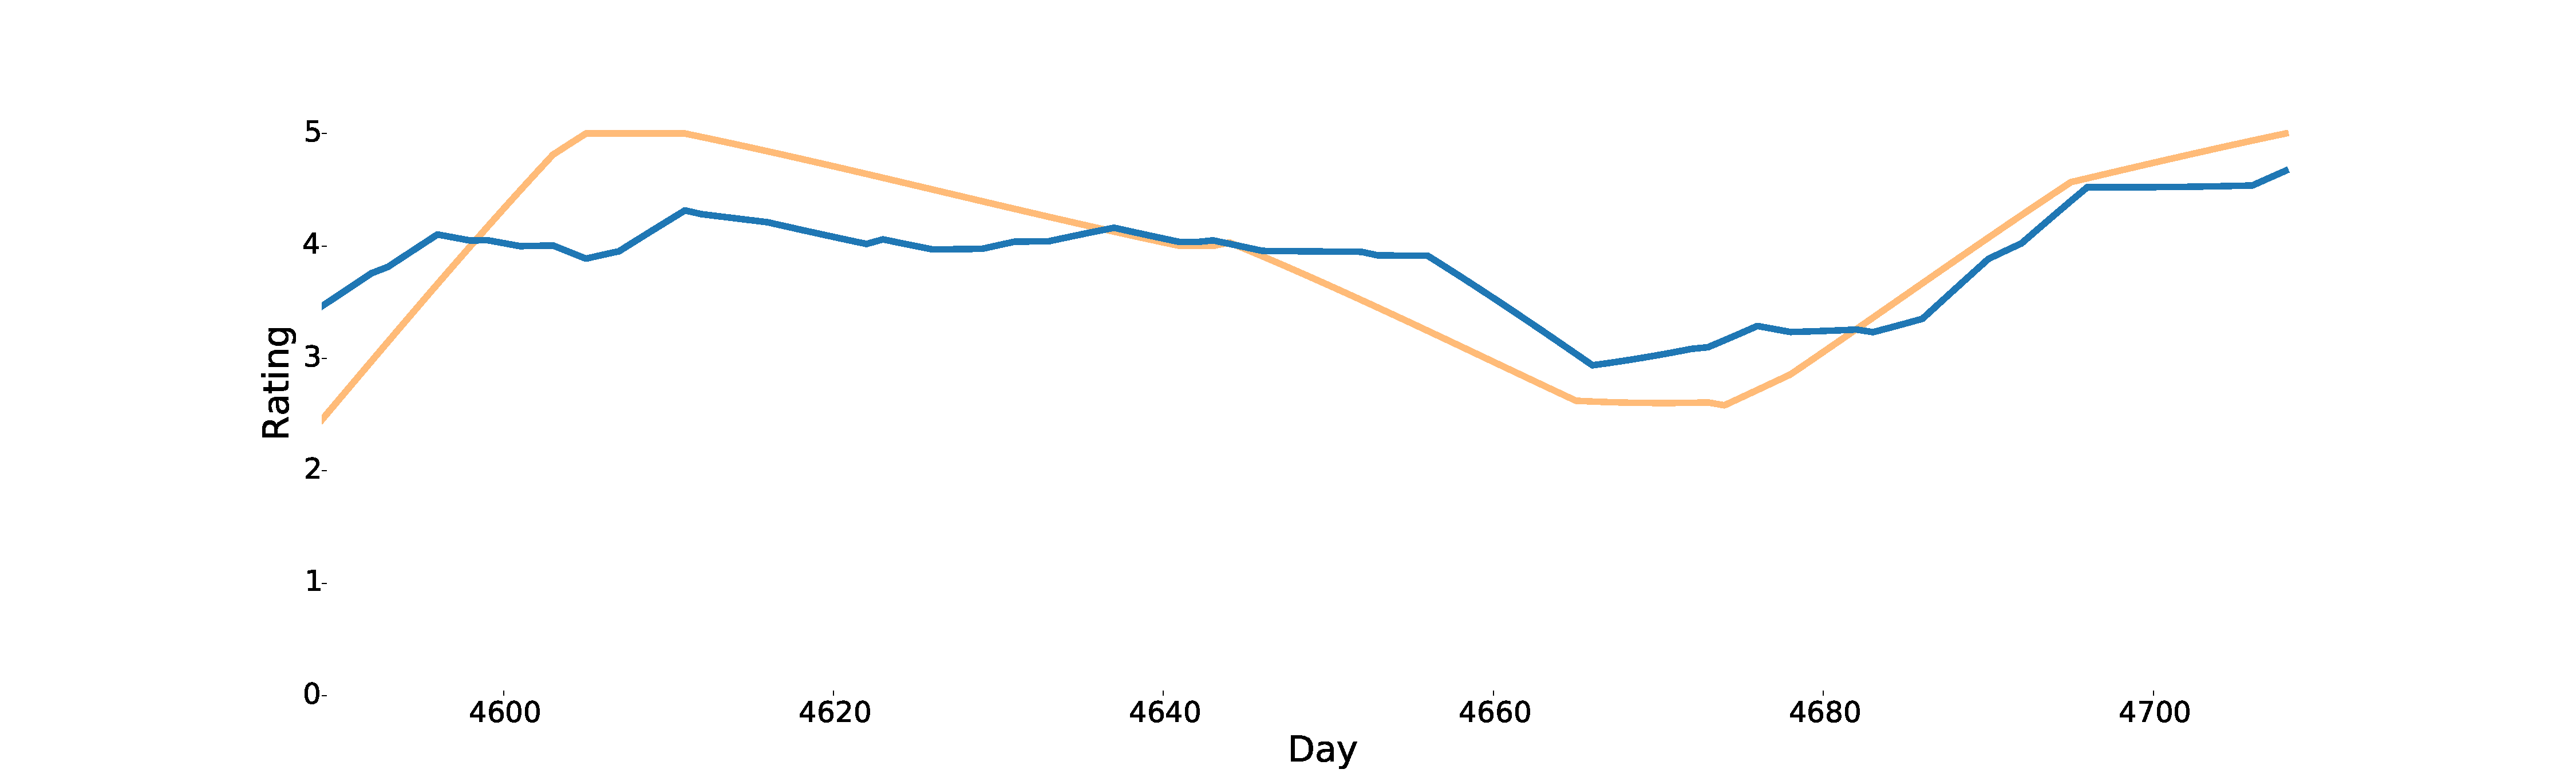
\includegraphics[width=\columnwidth]{corr.pdf}
\caption{Example of correlation analysis for a pair of businesses}
\end{figure}

\textbf{\textit{Hypothesis}} : None of the previous approaches provided an adequate metric.
For our last model we opted to use a correlation metric which reflects the relationship of two businesses over a long period of time.\\
\textbf{\textit{Proxy}} : Compute the correlation of ratings over time.\\
\textbf{\textit{Expected results}} : The correlation can be predicted using the attributes of the existing businesses and the new business. 

%----------------------------------------------------------------------------------------
%	RESULTS 
%----------------------------------------------------------------------------------------

\section*{Results}
%
The following table contains the mean training score and the 10-fold cross-validation score for predictions in a single cluster.
The cluster consists of 147 businesses which corresponds to 10730 pairings.
We did two types of experiments: (a) classification of positive vs. non-positive outcomes for all models and (b) classification of significant vs. insignificant outcomes (absolute value bigger than a certain threshold) for all models.

\begin{table*}[ht!]
\centering
\begin{tabular}{@{}llrrrr@{}}
\toprule
                                                              &                     & \multicolumn{2}{c}{sig/insig classif.} & \multicolumn{2}{c}{pos/neg classif.} \\ 
\cmidrule(r){3-4}
\cmidrule(r){5-6}
                                                              &                     & \multicolumn{1}{c}{60 days} & \multicolumn{1}{c}{90 days} & \multicolumn{1}{c}{60 days} & \multicolumn{1}{c}{90 days} \\ \midrule
\multirow{2}{*}{Conditional Mean}  & SVM rbf             &   0.84/0.61   &  0.82/0.60  & 0.84/0.60 &  0.85/0.65  \\
                                        & Logistic Regression & 0.61/0.52  & 0.60/0.52 &  0.56/0.49   &  0.56/0.49   \\ \midrule
\multirow{2}{*}{Trend Analysis}       & SVM rbf             & 0.83/0.62    &  0.82/0.59 & 0.84/0.60 & 0.81/0.58   \\
                                        & Logistic Regression &  0.60/0.55   & 0.58/0.48 &  0.57/0.49  &  0.56/0.51   \\ \midrule
\multirow{2}{*}{General Trend Analysis} & SVM rbf             & 0.84/0.62 & 0.80/0.62 &  0.81/0.60 &  0.83/0.63  \\
                                       & Logistic Regression &  0.59/0.52  & 0.58/0.54  &   0.57/0.49  &   0.58/0.49       \\ \midrule
\multirow{2}{*}{Correlation Analysis}   & SVM rbf             & \multicolumn{2}{c}{0.85/0.81}  & \multicolumn{2}{c}{0.86/0.81} \\
                                        & Logistic Regression & \multicolumn{2}{c}{0.84/0.82}  & \multicolumn{2}{c}{0.86/0.83} \\
\bottomrule
\end{tabular}
\caption{Training and 10-fold cross-validation score for predictions}
\end{table*}

\textit{Note}: We do not present the results for linear, poly and sigmoid kernels because the results were significantly worse than SVM with the rbf kernel.

\section{Conclusion}
We tried to predict the interaction of two businesses with multiple models.
The quality of our predictions turned out to be relatively low for most models.
Possible reasons are:
\begin{itemize}
\item The rating data is noisy and sparse at the same time. Most businesses don't have ratings every day and the variance of the ratings for a given time period is high.
\item The training score of SVM is high in general but the cross-validation score is low in a lot of cases which may be a hint that SVM is overfitting.
\item For the conditional mean analysis and the trend analysis, we assume that the opening date of the business is close to the first review submitted for the business. This might not always be the case.
\end{itemize}

We achieved good results when predicting correlation and this shows that our approach has merit.
We also observed that SVM generally outperformed logistic regression in cases other than correlation analysis.

\section{Future Work}
We have already performed different types of clustering on the data and chose the best one based on the geographical location of the businesses. It would be interesting to perform other types of clustering techniques based on the features distance metrics described in the features section, and study how the correlated businesses are geographicly located. This would allow us to analyze the structure of a cluster, e.g. whether a given cluster consists of many similar businesses (for example Chinatown in San Francisco) or whether a cluster is heterogenous (for example the Great Mall).\\
Since we have used very common business attributes like geographic distance, open hours, business types, and similar common features for our studies, we have the advantage to do the same experiments on similar datasets. In the future, it would be interesting to see if similar or even better observations can be made on different datasets, where more information on the businesses is available. In addition it would be interesting to look interactions between businesses other than the opening of a new business.

% The following two commands are all you need in the
% initial runs of your .tex file to
% produce the bibliography for the citations in your paper.
\bibliographystyle{abbrv}
\bibliography{main}  % vldb_sample.bib is the name of the Bibliography in this case

\end{document}
